%% This is file `elsarticle-template-1-num.tex',
%%
%% Copyright 2009 Elsevier Ltd
%%
%% This file is part of the 'Elsarticle Bundle'.
%% ---------------------------------------------
%%
%% It may be distributed under the conditions of the LaTeX Project Public
%% License, either version 1.2 of this license or (at your option) any
%% later version.  The latest version of this license is in
%%    http://www.latex-project.org/lppl.txt
%% and version 1.2 or later is part of all distributions of LaTeX
%% version 1999/12/01 or later.
%%
%% The list of all files belonging to the 'Elsarticle Bundle' is
%% given in the file `manifest.txt'.
%%
%% Template article for Elsevier's document class `elsarticle'
%% with numbered style bibliographic references
%%
%% $Id: elsarticle-template-1-num.tex 149 2009-10-08 05:01:15Z rishi $
%% $URL: http://lenova.river-valley.com/svn/elsbst/trunk/elsarticle-template-1-num.tex $
%%

%\documentclass[preprint,authoryear,review,12pt]{elsarticle}
\documentclass[final,5p,times,twocolumn]{elsarticle}

%% Use the option review to obtain double line spacing
%% \documentclass[preprint,review,12pt]{elsarticle}

%% Use the options 1p,two column; 3p; 3p,twocolumn; 5p; or 5p,twocolumn
%% for a journal layout:
%% \documentclass[final,1p,times]{elsarticle}
%% \documentclass[final,1p,times,twocolumn]{elsarticle}
%% \documentclass[final,3p,times]{elsarticle}
%% \documentclass[final,3p,times,twocolumn]{elsarticle}
%% \documentclass[final,5p,times]{elsarticle}
%% \documentclass[final,5p,times,twocolumn]{elsarticle}


\usepackage{color}
\usepackage{multirow,booktabs,ctable,array}
\usepackage{lscape}
\usepackage{amsmath}
\usepackage{lineno}
\usepackage{ulem}
\usepackage{setspace}
\usepackage{listings}
\usepackage{float}
\usepackage{listings}
\usepackage{color,colortbl}
\usepackage{rccol}
%\usepackage[table]{xcolor}

    \definecolor{listcomment}{rgb}{0.0,0.5,0.0}
    \definecolor{listkeyword}{rgb}{0.0,0.0,0.5}
    \definecolor{listnumbers}{gray}{0.65}
    \definecolor{listlightgray}{gray}{0.955}
    \definecolor{listwhite}{gray}{1.0}
    \definecolor{lightcyan}{rgb}{0.88,1,1}

\newcommand{\lstsetcpplong}
{
\lstset{frame = tb,
        framerule = 0.25pt,
        float,
        fontadjust,
        backgroundcolor={\color{listlightgray}},
        basicstyle = {\ttfamily\scriptsize},
        keywordstyle = {\ttfamily\color{listkeyword}\textbf},
        identifierstyle = {\ttfamily},
        commentstyle = {\ttfamily\color{listcomment}\textit},
        stringstyle = {\ttfamily},
        showstringspaces = false,
        showtabs = false,
        numbers = none,
        numbersep = 6pt,
        numberstyle={\ttfamily\color{listnumbers}},
        tabsize = 2,
        language=,
        floatplacement=!h,
        caption={\small \baselineskip 12pt DiReCT long command line menu which is invoked using the `{\ttfamily {-}{-}help}' option.  The short command line menu is obtained by typing `{\ttfamily {-}h}'},
        captionpos=b,
        label=listing:long
        }
}

\floatstyle{plain}
\newfloat{command}{thp}{lop}
\floatname{command}{Command}

%\usepackage[nomarkers,notablist]{endfloat}

%% if you use PostScript figures in your article
%% use the graphics package for simple commands
%% \usepackage{graphics}
%% or use the graphicx package for more complicated commands
%% \usepackage{graphicx}
%% or use the epsfig package if you prefer to use the old commands
%% \usepackage{epsfig}

%% The amssymb package provides various useful mathematical symbols
\usepackage{amssymb}
%% The amsthm package provides extended theorem environments
% \usepackage{amsthm}
 
 \usepackage{makecell}

%% The lineno packages adds line numbers. Start line numbering with
%% \begin{linenumbers}, end it with \end{linenumbers}. Or switch it on
%% for the whole article with \linenumbers after \end{frontmatter}.
%% \usepackage{lineno}

%% natbib.sty is loaded by default. However, natbib options can be
%% provided with \biboptions{...} command. Following options are
%% valid:

%%   round  -  round parentheses are used (default)
%%   square -  square brackets are used   [option]
%%   curly  -  curly braces are used      {option}
%%   angle  -  angle brackets are used    <option>
%%   semicolon  -  multiple citations separated by semi-colon
%%   colon  - same as semicolon, an earlier confusion
%%   comma  -  separated by comma
%%   numbers-  selects numerical citations
%%   super  -  numerical citations as superscripts
%%   sort   -  sorts multiple citations according to order in ref. list
%%   sort&compress   -  like sort, but also compresses numerical citations
%%   compress - compresses without sorting
%%
%% \biboptions{comma,round}

% \biboptions{}

\providecommand{\OO}[1]{\operatorname{O}\bigl(#1\bigr)}

\graphicspath{
             {./Figures/}
             }

\long\def\symbolfootnote[#1]#2{\begingroup%
\def\thefootnote{\fnsymbol{footnote}}\footnote[#1]{#2}\endgroup}



\journal{NeuroImage}

\begin{document}


\begin{frontmatter}

\title{Multivariate Neuroanalysis with ANTsR: Application to Supervised Brain Tumor Segmentation using Random Forests}

\author[label1]{Nicholas J.~Tustison
  \fnref{label0}}
  \fntext[label0]{\scriptsize Corresponding author:  PO Box 801339, Charlottesville, VA 22908; T:  434-924-7730; email address:  ntustison@virginia.edu.
  }
\author[label2]{K.~L.~Shrinidhi}
\author[label2]{Jeffrey T.~Duda}
\author[label1]{Christopher R.~Durst}
\author[label1]{Max Wintermark}
\author[label1]{James C.~Gee}
\author[label1]{Murray C.~Grossman}
\author[label2]{Brian B.~Avants}
\address[label1]{Department of Radiology and Medical Imaging, University of Virginia, Charlottesville, VA}
\address[label2]{Penn Image Computing and Science Laboratory, University of Pennsylvania,
                Philadelphia, PA}

%\maketitle

\linenumbers

\begin{abstract} 
Improvements in image acquisition and increasingly sophisticated statistical techniques 
for neuroanalysis have motivated the development of advanced computational software 
packages for studying the
brain---many of which
have been made publicly available.  One such popular toolkit is the open source Advanced
Normalization Tools (ANTs) which contains a suite of well-vetted processing tools for
core data transformation tasks such as image registration, image segmentation, 
inhomogeneity field correction, and template building.  Despite the numerous
solutions afforded by such packages, neuroscience (and data analysis in general) requires
robust, statistical tools for making predictive inferences with respect to given hypotheses
and for rendering quantitative information in clarifying and insightful ways.  
In this paper, we describe the
coupling of ANTs with the widely-used R language---an open source environment for 
statistical processing and data visualization---which we denote as ANTsR.  One of the
many benefits from such integration is the accessibility to advanced statistical 
and machine learning techniques as well as state-of-the-art visualization possibilities.  
To showcase the flexibility and utility of ANTsR, we 
apply it to the difficult problem of brain tumor segmentation from multi-modality
MRI.  The reported algorithmic framework was the top-performing entry in the MICCAI 2013 Multimodal 
Brain Tumor Segmentation (BRATS) challenge and, to our knowledge, is the only entry for
both challenge years (2012, 2013) which has been made publicly available as open source.
\end{abstract}

\begin{keyword}
advanced normalization tools \sep BRATS \sep brain tumor segmentation \sep R project \sep random forests
%% keywords here, in the form: keyword \sep keyword
\end{keyword}

\end{frontmatter}
%
%
\newpage

%% MSC codes here, in the form: \MSC code \sep code
%% or \MSC[2008] code \sep code (2000 is the default)

%%
%% Start line numbering here if you want
%%
% \linenumbers

%% The Appendices part is started with the command \appendix;
%% appendix sections are then done as normal sections
%% \appendix

%% \section{}
%% \label{}

%% References
%%
%% Following citation commands can be used in the body text:
%% Usage of \cite is as follows:
%%   \citep{key}          ==>>  [#]
%%   \cite[chap. 2]{key} ==>>  [#, chap. 2]
%%   \citet{key}         ==>>  Author [#]

%% main text

%\input{intro}
%
%\input{methods}

\section{Introduction}

ANTs (Advanced Normalization Tools) originated with the open source availing
of high-performance registration algorithms for neuroimage analysis
\citep{avants2008a} built upon the mature and well-vetted Insight Toolkit (ITK)
of the National Institutes of Health.  Since then, ANTs has grown to include 
several algorithmic solutions for robust medical image analysis including bias 
correction \citep{tustison2010}, $n$-tissue multivariate segmentation 
\citep{avants2011}, template construction \citep{avants2010}, and cortical 
thickness estimation \citep{das2009} (many of which have been
introduced into ITK partially in an attempted leveraging of Linus's Law---``Given enough eyeballs, all bugs are shallow'').  
However, in the evolution of the toolkit, it became clear 
that robust statistical machinery was lacking for making inferences regarding
the data produced during the course of ANTs processing.  ANTsR was developed
specifically to provide an interface between ANTs, a 
powerful neuroimaging toolkit for producing reliable imaging data 
transformations, and the R project%
\footnote{
http://www.r-project.org
}
for statistical computing and visualization thus providing a complete
set of tools for multivariate neuroimage analysis. 

In addition to describing ANTsR basics and how it can be
used generally in multivariate neuroimaging studies, we showcase its use in
the particularly difficult application of supervised brain tumor
segmentation \cite{bauer2013} for which we use the widely popular 
random forests machine learning technique.  Although random forests have
been proposed previously in the literature for, among other things, 
supervised brain segmentation (e.g. \cite{geremia2011}), 
we demonstrate that ANTsR significantly facilitates the construction 
of a fully functional, parallelizable workflow for such a task and 
that the performance of our proposed framework has proven extremely in 
actual practice, specifically
 in the recent MICCAI 2013 Multimodal Brain Tumor Segmentation
Challenge (see Figure \ref{fig:award}).%
\footnote{
http://martinos.org/qtim/miccai2013/
}
\begin{figure}
  \centering
  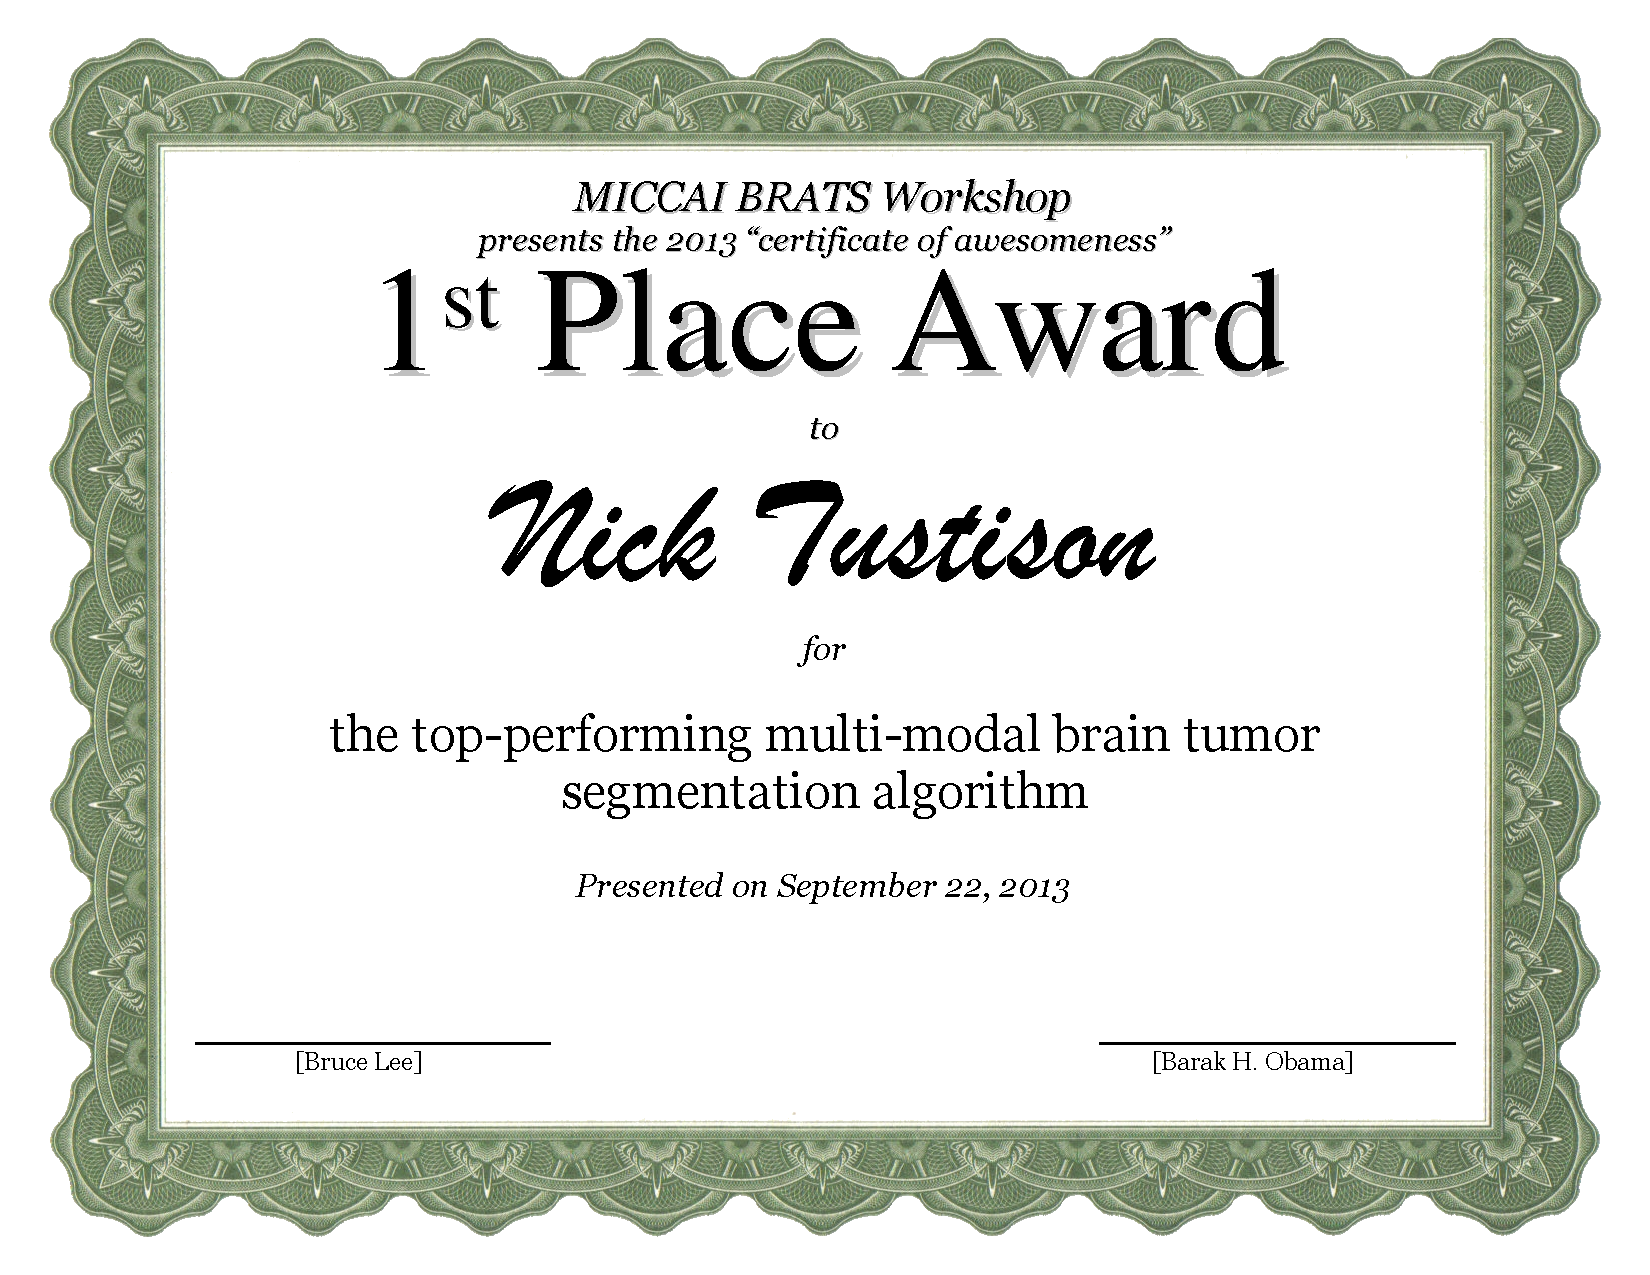
\includegraphics[width=80mm]{Figures/award.pdf}
  \caption{First place certificate from the MICCAI 2013 BRATS challenge.}
  \label{fig:award}
\end{figure}

It is interesting to note that our participation in the 2013 challenge
was the result of observing the 2012
challenge, wanting to take advantage of the same methods as the winners,
and finding that no teams had availed their software in any form.  In contrast, 
and very much in line with our philosophy 
regarding open science \citep{tustison2013,ince2012}, we have made this framework available as open 
source (even releasing the code before the actual 2013 contest).%
\footnote{
https://github.com/ntustison/BRATS2013
}
To our knowledge, we are the only competitors out of the 20 or so teams 
that participated in either years' challenges to do this.

\section{Materials and Methods}

\subsection{ANTsR:  An ANTs/R Interface}

\subsubsection{Overview}

The complexity of neuroimaging research necessitates 
commensurable numerical analysis capabilities.  Similarly, concomitant
with the era of ``big data'' (specifically with respect to neuroimaging
\citep{vanhorn2013}) are new visualization needs and challenges
\citep{childs2013,kehrer2013}.
In response, various software packages have been developed to
integrate tools specific to neuroimaging research with more general
numerical and visualization software packages.
The well-known neuroimaging de facto standard SPM%
\footnote{
http://www.fil.ion.ucl.ac.uk/spm/
}
is a significant extension of the commercial computing and visualization environment
Matlab.  Open source neuroimaging packages, such as NIPY (neuroimaging in Python),%
\footnote{
http://nipy.org
} 
rely on other open source packages for numerical/statistical analysis.  NIPY,
for example, uses the more generic packages NumPy and SciPy for numerical analysis and 
optimization.%
\footnote{
http://www.numpy.org
}  

Careful consideration of available options
led to the adoption of R to complement ANTs capabilities resulting in the
ANTsR package.
The R project for statistical computing,%
\footnote{
www.r-project.org
}
 or more compactly
`R', is an environment for statistical computation
and data visualization.  R's open source code base
and add-on packages coupled with its rapidly growing 
community of developers and users has caused wide-scale
adoption within both academia and industry.

\subsubsection{Installation}

The ANTsR package is publicly available on the github project hosting service.%
\footnote{
https://github.com/stnava/ANTsR
}
Prior to installation of ANTsR, several external R packages
need to be installed including: \verb#Rcpp#, \verb#signal#, \verb#timeSeries#, 
\verb#mFilter#, \verb#doParallel#, \verb#robust#, \verb#magic#, \verb#knitr#, \verb#pixmap#, 
\verb#rgl#, and \verb#misc3d#.  Additionally, in order
to perform the supervised brain segmentation as described 
in later sections, one needs to also install the packages
\verb#randomForest#, \verb#snowfall#, \verb#rlecuyer#,
and \verb#ggplot2#.%
\footnote{
Packages are easily installed using the {\tt install.packages()} R function.
} 

In addition to R and the add-on packages previously mentioned, CMake is also 
required.  CMake%
\footnote{
http://www.cmake.org/
}
is an open source tool for the management and building of 
large-scale software projects.  It is used
to coordinate the downloading of external packages,
such as the Insight Toolkit (ITK)%
\footnote{
http://www.itk.org/
}
and ANTs.  Further instructions for download and
installation can be found on the ANTsR github website.

\subsubsection{Usage}
The utility of ANTsR stems from the ability to couple ANTs core 
functionality, including IO tools such as \verb#antsImageRead#, 
with the large number of R statistical and
visualization packages.  Due to this combination, several
functions have been easily created for such neuroimaging-specific 
tasks as fMRI/ASL data manipulation and analysis,
voxel and ROI-based  analyses,
%(e.g. \verb#filterMRIforNetworkAnalysis#, \verb#aslPerfusion#)
and connectivity visualization. % (e.g. \verb#plotBasicNetwork#).
The user help menu and documentation for the library  and its
constituent functions are invoked in the similar manner as other
R libraries.

\subsection{Supervised Brain Tumor Segmentation with Random Forests}

Supervised techniques generally consist of a training phase
for model construction followed by prediction using the previously
generated model.  For supervised brain tumor segmentation, 
a set of training data consisting of labeled brain images 
(e.g. csf, gray matter, white matter, 
necrosis, edema, enhancing and  non-enhancing tumor) is
used to construct a predictive model.  Although other 
classification techniques have been used to segment
brain tumors (e.g. support vector machines \citep{bauer2011}),
random forest models have proven particularly successful.

In subsequent sections, we detail the generic
random forest modeling framework which takes as input
a set of feature images (also described in a later section)
and labels for each training subject 
and outputs a statistical model.  This model, in turn, can then
be used to provide a probabilistic estimate of the labels in an
unlabeled subject. 

%One of the core extensions that we provide in this work is
%the use of concatenated random forests for improved probabilistic estimation
%of the labels.
%As we demonstrate in the Results section, the set of feature
%images employed work sufficiently well for good performance
%on the training data.  However, we discovered
%that further improvements could be gained by using the probabilistic 
%label estimates as input to enhance preprocessing before a 
%second round of feature image generation including 
%modality-specific, prior-based $n$-tissue segmentation and 
%random forest model creation. 

Several machine learning concepts were integrated to create 
the random forests framework first articulated in its entirety by Breiman
et al. \cite{breiman2001} for performing classification/regression.  
Although decision trees had been previously explored in the literature, 
it was the success of ``boosting''-style machine learning 
techniques, such as AdaBoost \cite{schapire1990,freund1997}, which influenced 
the aggregation of such decision trees into ``forests'' 
with randomized node optimization for improved
classification/regression performance \cite{ho1995,amit1997}.
The final element of bootstrap aggregating or ``bagging'' (i.e.
random sampling of the training data) was
introduced by Breiman \cite{breiman1996} to achieve improved
accuracy.  

Early adoption \cite{viola2005} and success in the
computer vision community
has led to a recent surge within the medical image analysis
community of using random forests for handling complex 
classification/regression tasks including
normal brain segmentation \cite{yi2009},
MS lesion segmentation \cite{geremia2011}, 
multimodal brain tumor segmentation
\cite{bauer2012,zikic2012}, brain extraction \cite{iglesias2010}, 
anatomy detection in computed tomography \cite{criminisi2013}, and
segmentation of echocardiographic images \cite{verhoek2011}. 
A thorough introduction for those interested in delving deeper 
into the more theoretical aspects of random forests can be found
in \cite{criminisi2011}.

One of the principal advantages of R is the extensive community of
developers  who have contributed on the order of thousands of packages 
extending R's capabilities beyond its core functionality.
Most relevant for the work described in this paper
is the \verb#randomForest# package developed from Breiman's original
Fortran code by Liaw and Wiener \citep{liaw2002}.


\subsubsection{Brain Tumor Data}

Brain tumor image data used in this work were obtained from the NCI-MICCAI 2013 
Challenge on Multimodal Brain Tumor Segmentation%
\footnote{
http://martinos.org/qtim/miccai2013/index.html
}
organized by K. Farahani, M. Reyes,B. Menze, E. Gerstner, J. Kirby and J. Kalpathy-Cramer. The challenge database contains fully anonymized images from the following institutions: 
ETH Zurich, University of Bern, University of Debrecen, and University of Utah and 
publicly available images from the Cancer Imaging Archive (TCIA).  Both training 
and testing data were made freely available through the Creative Commons Attribution-NonCommercial 3.0 license.

Training data consisted of multi-modal brain MRI (T1, T2, FLAIR, and 
post-Gadolinium T1) from 30 glioma patients (both low, $n=10$, and high-grade, $n=20$,
and with and without resection).  For each subject, the T1, T2, and 
FLAIR MRI were linearly registered to the post-contrast T1.  Subsequently,
the brains were skull-stripped and resampled to 1 mm isotropic resolution.
Testing data was processed similarly and released during the course of the
challenge in two sets denoted as ``LeaderBoard'' and ``Challenge'' data.  
The former consisted of 21 and 4 high and low-grade tumor patients, respectively,
whereas the latter comprised 10 high-grade only patients.

Manual labeling was performed in the axial plane following a detailed
protocol.%
\footnote{
http://martinos.org/qtim/miccai2013/data.html.
}
The labeling of pathology was categorized into four regions:
edema, non-enhancing tumor (including low-grade tumor center), 
enhancing tumor (excluding necrotic center), and abnormal
necrotic center or necrocyst in high-grade gliomas.
Normal brain tissue was not labeled. 

%\subsubsection{Multi-Modal Feature Image Preprocessing}
%Although several studies have pointed out the importance of
%intensity normalization and bias correction, our experience 
%with the training data illustrated a degradation in performance
%when one or both steps (using \cite{nyul2000} and N4 \cite{tustison2010},
%respectively) were performed due to the presence of the tumor/edema complex. 
% 
%As a corrective, for the first stage we simply windowed the image intensity
%for all images to be between the quantiles $[0.01,0.99]$ and
%subsequently rescaled to $[0,1]$.  From these ``corrected'' images,
%the first set of feature images were derived.  For the training cohort, these
%data were used to create the random forest regression model for the first
%stage.  During the second stage, the probabilistic estimates
%of the white matter and gray matter labels were used to generate a
%``pure tissue weight mask'' to estimate the bias field 
%using N4 (although the resulting bias field estimation was used
%to correct the image within the entire cerebral mask).  Formally, this 
%involved generation of a probabilistic map defined as:
%\begin{align}
%  P_{pure\,\,tissue}(\mathbf{x}) = \sum_{i=1}^N P_i(\mathbf{x}) \prod_{j=1, j \neq i}^N \left( 1 - P_j(\mathbf{x}) \right)
%\end{align}
%where $N$ is the set of user-selected tissue labels (in our
%case $N=2$ consisting of the gray and white matter probability
%maps).
%
%Both rescaling and weighted bias correction were applied to produce
%the ``corrected images'' for the second stage resulting in
%modified features images for the second stage.  Note that we
%perform a similar iterative scenario for normal brain 
%segmentation \cite{avants2011} (encapsulated in the ANTs script 
%\verb#antsAtroposN4.sh#).

\subsubsection{Symmetric Multivariate Template Construction}

\begin{figure}
  \centering
  \begin{tabular}{cc}
    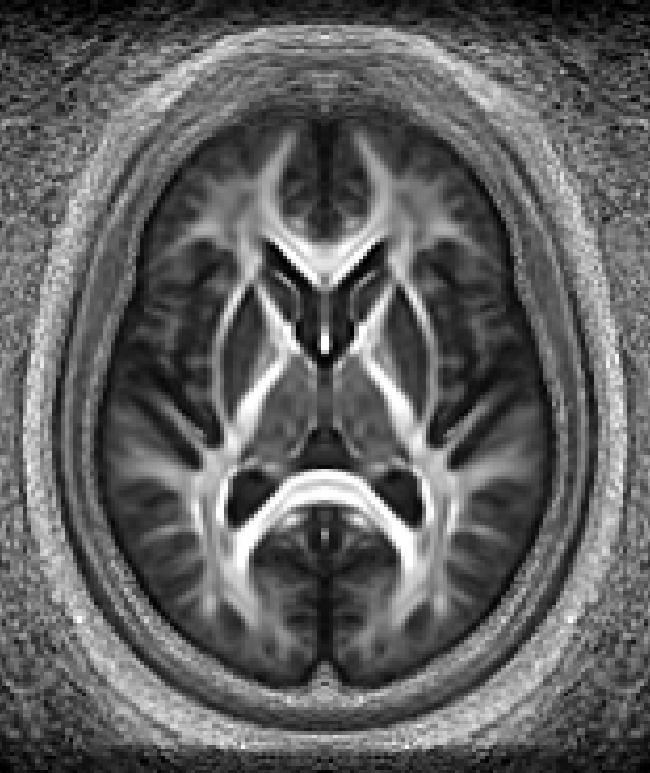
\includegraphics[width=40mm]{Figures/S_templateFA_140.png} &
    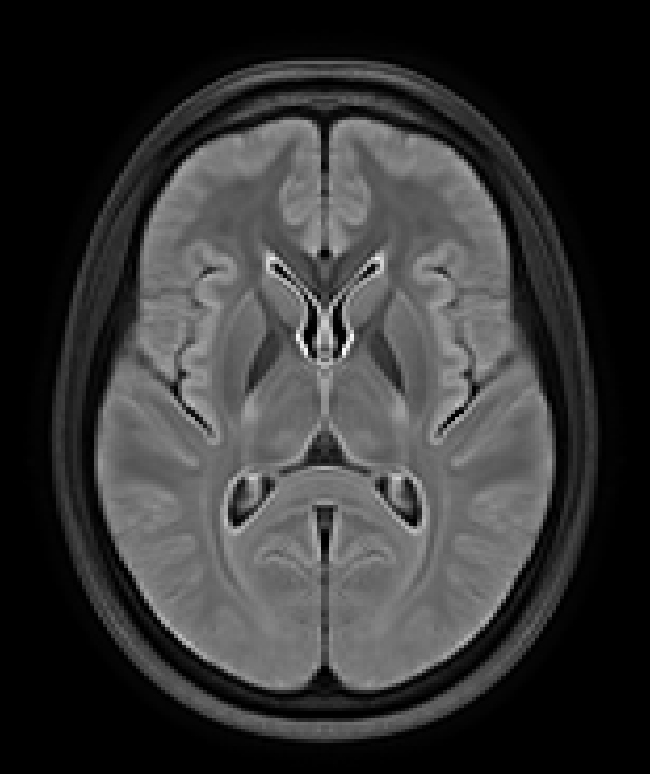
\includegraphics[width=40mm]{Figures/S_templateFLAIR_140.png} \\
    (a) & (b) \\
    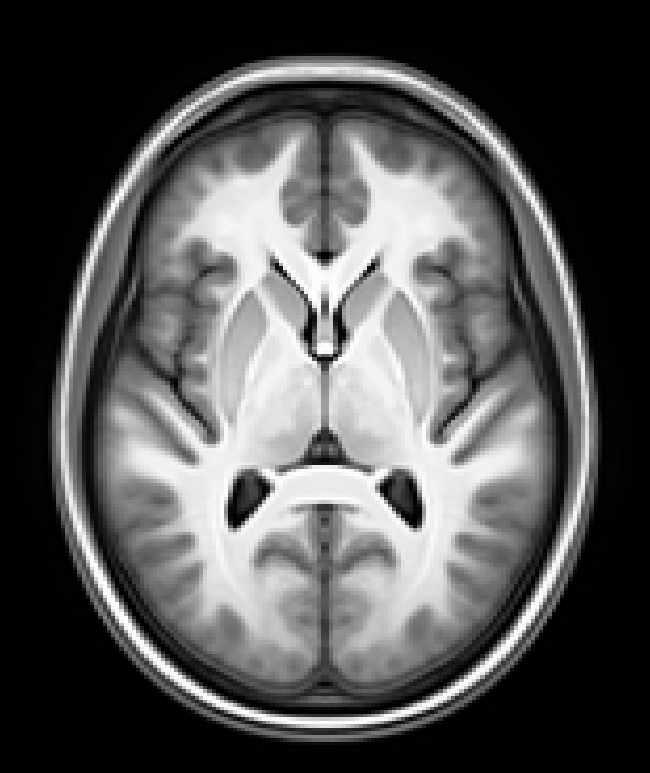
\includegraphics[width=40mm]{Figures/S_templateT1_140.png} &
    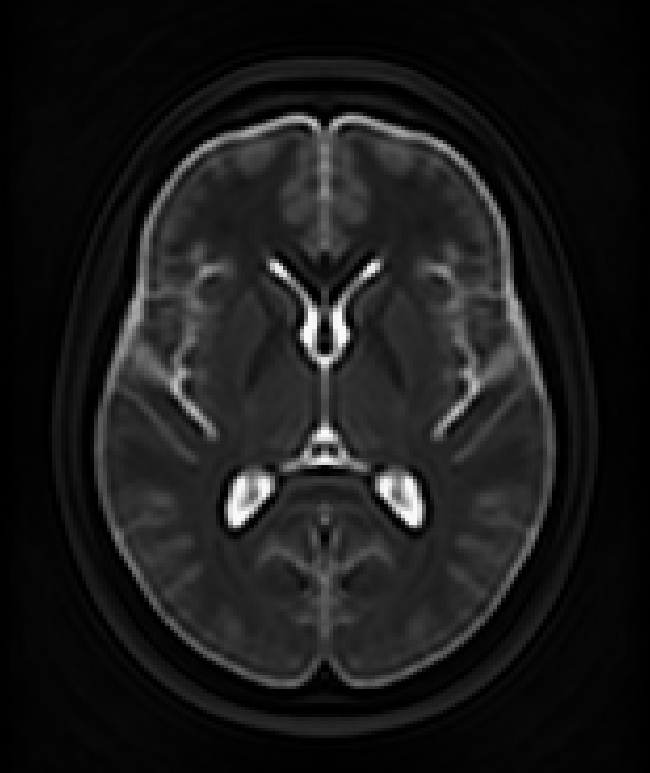
\includegraphics[width=40mm]{Figures/S_templateT2_140.png} \\
    (c) & (d) 
  \end{tabular}
  \caption{Multivariate symmetric template created from the Kirby 
           21 data described in \cite{landman2011}.  Shown are the
           (a) fractional anisotropy (FA), (b) FLAIR, (c) MPRAGE, 
           and (d) T2 template components.
          }
  \label{fig:symmetrictemplates}
\end{figure}

In order to better characterize deviations from normal
multi-modal brain shape and appearance, several features were derived 
using population-specific multivariate template 
construction. A recent neuroimaging reproducibility study
by Landman et al. resulted in an open data cohort of 21
normal individuals, each imaged twice, comprising several
modalities including ASL, FLAIR, DTI, fMRI, T1, and T2 
\cite{landman2011}.  These data (known informally as the
``Kirby'' data set) were selected for deriving
a multivariate template due to its public availability and
inclusion of several modalities (even permitting future 
incorporation into our segmentation framework of modalities 
not currently included with the BRATS challenge).

As detailed in \cite{avants2008,avants2010}, 
given $K$ image modalities for $N$ subjects,  
${\mathbf I} = \{I_1,I_2,\ldots, I_K\}$, multivariate 
template construction iterates between optimizing the set 
of diffeomorphic transforms between the subjects and the 
template, 
$\left\{\left(\phi_1,\phi_1^{-1}\right),\ldots,\left(\phi_N,\phi_N^{-1}\right)\right\}$ 
and constructing the 
optimal multivariate template appearance 
$\mathbf{J}=\{J_1,J_2,\ldots, J_K\}$ to minimize the
following cost function:
\begin{align}
  \sum_{n=1}^N 
        \Bigg[ D &\left( \psi(\mathbf{x}),\phi_1^n(\mathbf{x},1)\right) \\ \nonumber 
        +& \sum_{k=1}^K \lambda_k \Pi_k \left(I_k^n\left(\phi_n(\mathbf{x},0.5)\right),J_k\left(\phi^{-1}_n(\mathbf{x},0.5)\right)\right)\Bigg].
\end{align}
$D$ is the diffeomorphic shape distance,
\begin{align}
D\left( \phi( \mathbf{x},0),\phi( \mathbf{x},1)\right) = \int_0^1 \| \nu(\mathbf{x},t)\|_L dt
\end{align}
dependent on the choice of linear operator, $L$, and $\nu$
is the velocity field
\begin{align}
\nu\left( \phi(\mathbf{x},t) \right) = \frac{d\phi(\mathbf{x},t)}{dt},\,\,\, \phi(\mathbf{x},0) = \mathbf{x}.
\end{align}
Each pairwise registration employing the similarity metric $\Pi_k$ can 
be assigned a relative weighting, $\lambda_k$, to weight a particular
modality's influence in the construction process.  

In terms of implementation, this algorithm is 
encapsulated in the script \verb#antsMultivariateTemplateConstruction.sh#,
available in the ANTs repository, which permits parallel processing on
an individual workstation or on a large computational cluster.  In
Figure \ref{fig:symmetrictemplates} we show mid-axial slices from
the Kirby multivariate symmetrical template consisting of FA, FLAIR,  
T1, and T2 components.  Although DTI-based images were not included in the
challenge data, such images have shown discriminative potential 
\citep{price2003} to warrant investigation in our future work.

\subsubsection{Multi-Modal Feature Image Generation}

\begin{figure*}
  \centering
  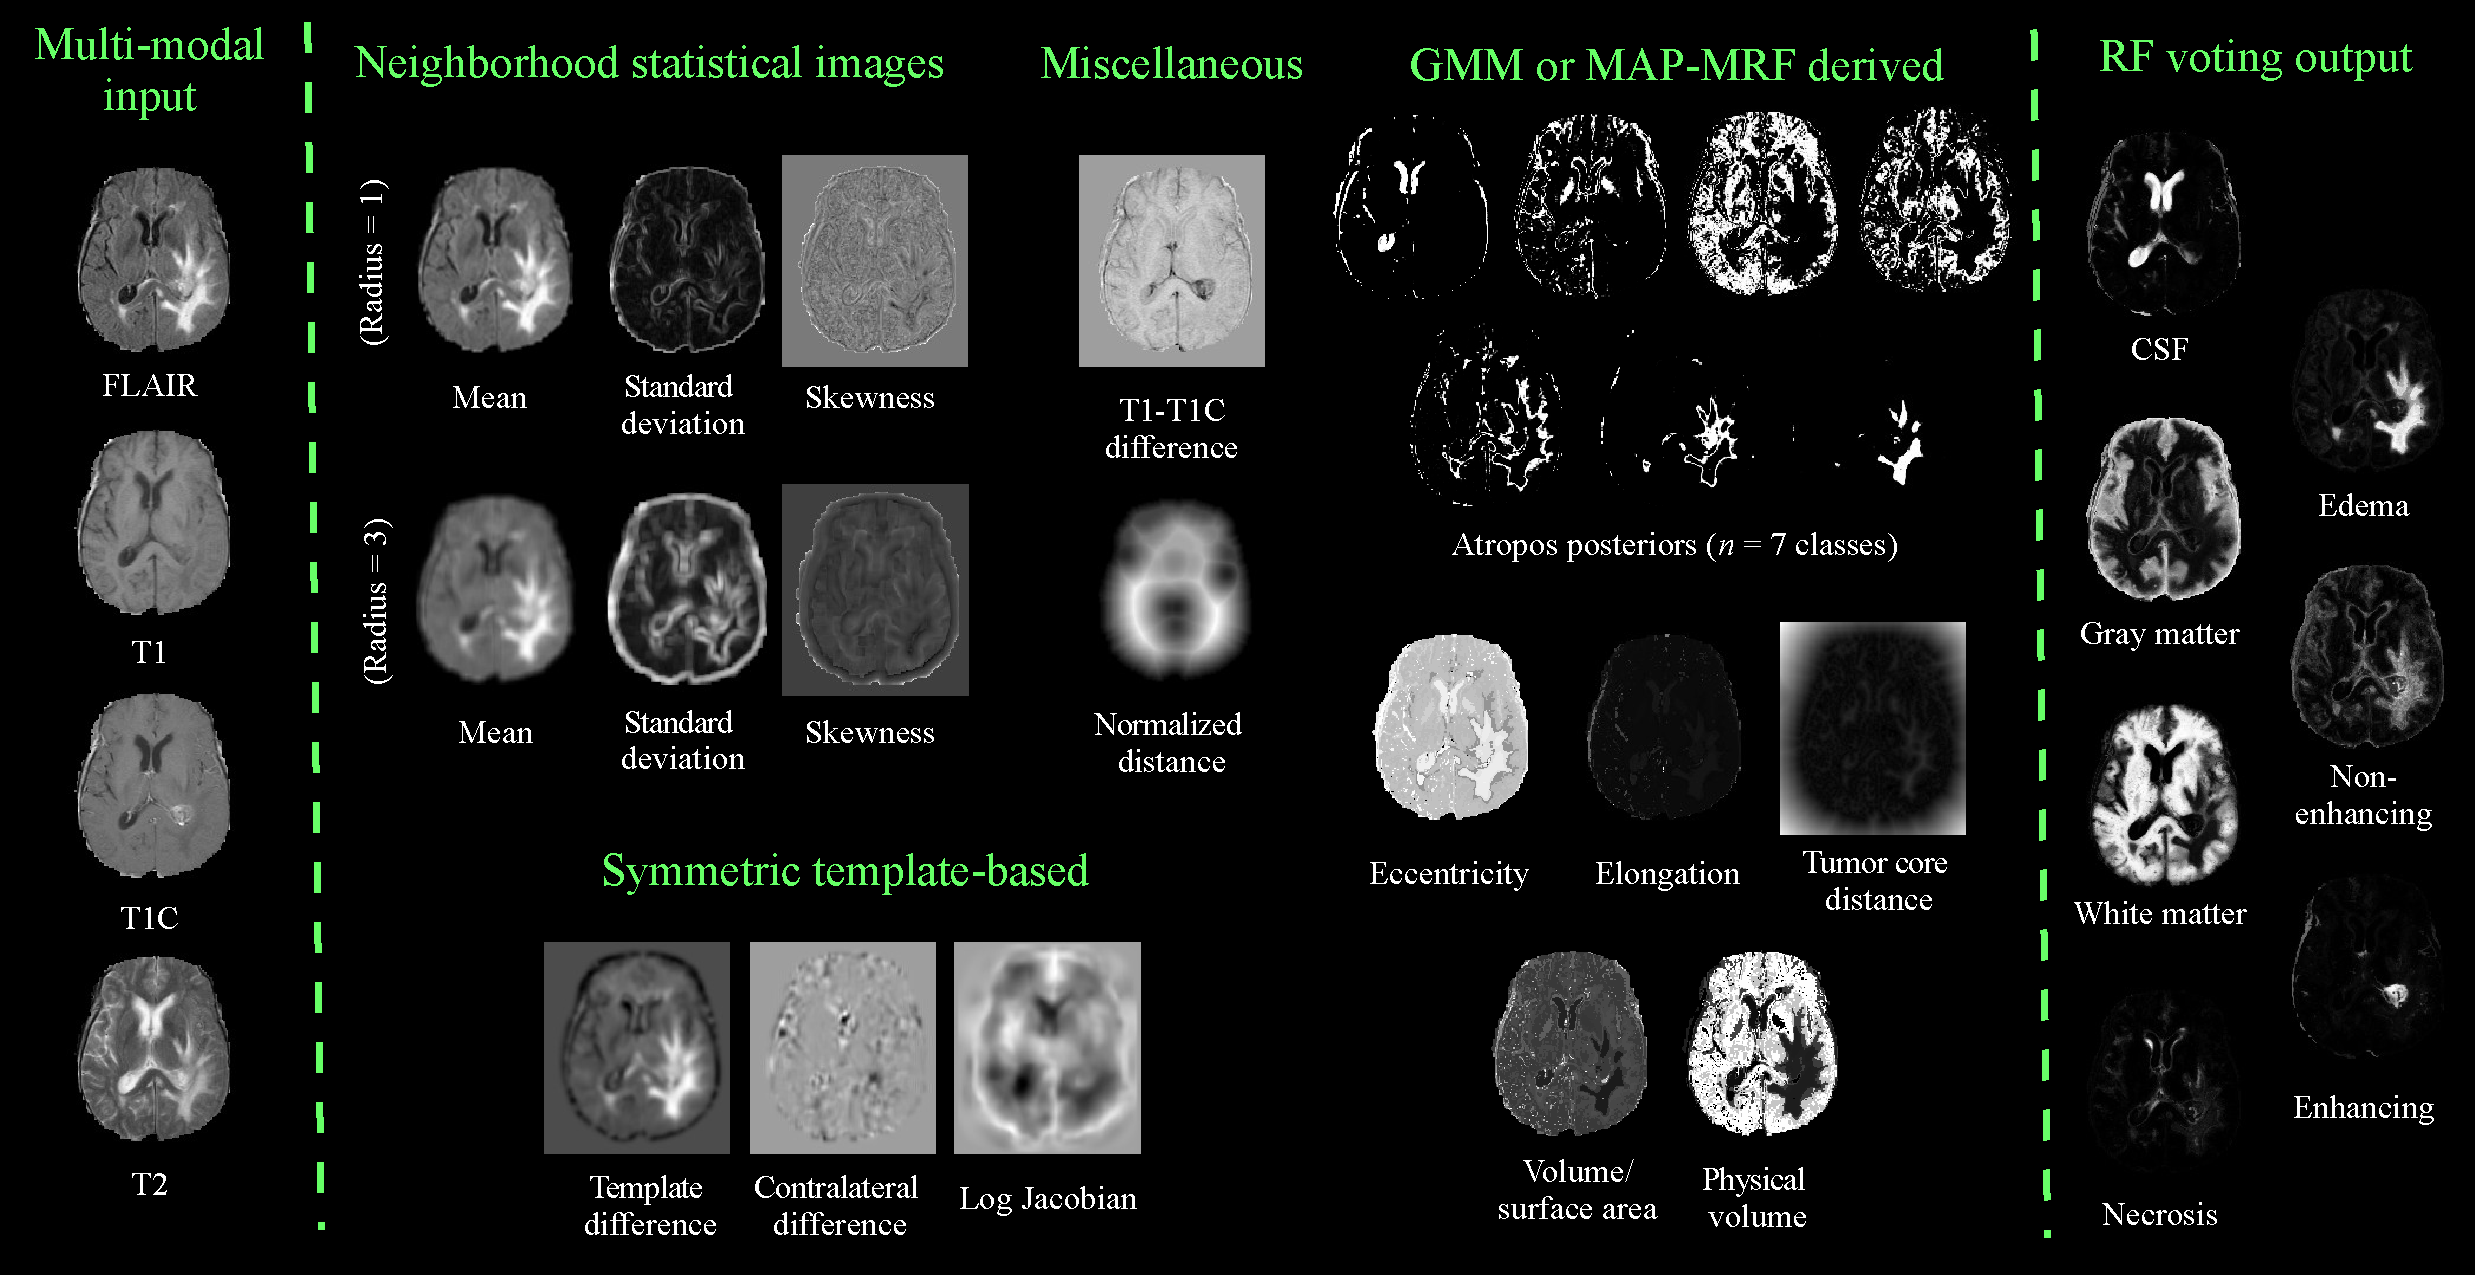
\includegraphics[width=180mm]{Figures/featureImages.pdf}
  \caption{Representative feature images derived from the BRATS\_HG0301 ``challenge'' data set.
           Neighborhood statistical images for each modality were generated by calculating a 
           given statistic within
           a specified neighborhood radius.  Also calculated for each modality were feature
           images based on either the GMM or the MAP-MRF segmentation.  For the former, we
           show the probability maps for each of the seven labels which are used as feature
           images.  From the resulting hard segmentation, we calculate various geometric 
           measures per connected component of each of the seven labels.  Similarly, the 
           registration to the symmetric template produces the modality-specific difference images with the
           corresponding symmetric template itself and with respect to the contralateral side.   
           This mapping is also used to produce the log Jacobian image.  Finally, the T1 - TC image
           is calculated and, from the
           cerebral mask, we calculate the normalized distance image.  
           }
\end{figure*}

The workflow for estimating tumor-based labeling from multi-modal 
images involves the following steps:
\begin{enumerate}
  \item Symmetric multivariate template construction \cite{avants2010}
 using the data described in \cite{landman2011}.
  \item Image preprocessing:
    \begin{itemize}
      \item Windowing intensities (quantiles $[0.01,0.99]$).
      \item N4 bias correction \cite{tustison2010}.
      \item Rescaling intensity range to $[0,1]$.  
    \end{itemize}
  \item Stage 1 (GMM) processing:
  \begin{itemize}
    \item generation of feature images,
    \item construction of the Stage 1 RF model and probability images.
  \end{itemize}
  \item Stage 2 processing:
  \begin{itemize}
    \item generation of single-modality MAP-MRF images using the Stage 1 RF probability images as spatial priors,
    \item construction of the Stage 2 RF model and labelings.
  \end{itemize}
  \item Refinement of Stage 2 labelings using a heuristically-derived binary morphological processing protocol.
\end{enumerate}

Key to any supervised regression or classification protocol are the 
selected features for training and subsequent prediction.  Based on previous
work and our own experience, the following feature images were selected:
\begin{itemize}
  \item Per modality (FLAIR, T1, T1C, T2)
    \begin{itemize}
      \item First-order neighborhood statistical images:
            mean, variance, skewness, and entropy. 
            Neighborhood radius $\in \{1,3\}$.
    \item GMM (stage 1) and MAP-MRF (stage 2) posteriors: CSF, gray matter, white 
          matter, necrosis, edema, non-enhancing tumor and enhancing tumor (or a
          subset for the simulated data).
    \item GMM (stage 1) and MAP-MRF (stage 2) connected component geometry 
          features:  distance to tumor core label, volume, volume to surface area ratio, eccentricity, and elongation
    \item Template-based:  symmetric template difference and 
          contralateral difference with Gaussian smoothing ($\sigma = 4$mm).
    \end{itemize}
  \item Miscellaneous: normalized Euclidean distance based on cerebral mask,
    log Jacobian image, and  (T1C - T1) difference image.
\end{itemize}






For each modality, we create four first-order statistical feature images,
five Gaussian mixture model (GMM)-based posterior probability feature images,
four geometry features generated from the GMM posterior probability images
based on connected components, and two difference images using symmetric template
construction for a total of 4 modalities $\times$ (4 + 5 + 4 + 2) feature images per modality $=$ 60 total
feature images.  We employ two additional images consisting of the 
Euclidean distance image \cite{maurer2003} created from the skull-stripped 
binary mask rescaled to the range $[0,1]$ and the log
Jacobian image derived from the spatial normalization of the symmetric multivariate template and individual subject images.  Given the intensity corrected images
the corresponding multivariate template images, and a brain mask for each subject
creation of all feature images is performed using the script \verb#createFeatureImages.sh#.

Prior  cluster centers for specific tissue types learned from training data \cite{reynolds2009} are used in the GMM to create multiple feature images.  
Given $M$ tissue types (e.g. CSF, gray matter,
white matter, edema, and tumor), a GMM formulates the 
probability distribution at each voxel, $\mathbf{x}$, as the
sum of Gaussian components, $\mathcal{N}(\mathbf{x}|\mu,\sigma)$, i.e.
\begin{align}
p\left(\mathbf{x}|\mu_m,\sigma_m,\lambda_m\right) = \sum_{i=1}^M \lambda_m \mathcal{N}(\mathbf{x}|\mu_m,\sigma_m)
\end{align}
where $\sum_{m=1}^M \lambda_m = 1$.  One popular method for 
determining the parameters of the GMM is maximum likelihood 
estimation which can performed using the Atropos segmentation 
tool \cite{avants2011}.  In contrast to previous generative
modeling approaches for multi-modal tumor segmentation 
(e.g. \cite{prastawa2003}), we do not use multivariate 
Gaussians to specify tissue probabilities but rather incorporate each
univariate probability map into the feature vector of the training
data.  As pointed out in \cite{menze2010}, multivariate modeling
might obscure the distinct biological information provided by each 
modality.  Instead, we let the random forest construction 
process determine the optimal combination of such multivariate
information.
Additionally, maximum posterior labeling from the GMM processing
is used to determine the connected components for each label.  
Geometric features (assigned voxel-wise) include the physical volumes 
of each connected component including the volume to surface area ratio, 
the elongation, and eccentricity. 



\subsubsection{Training:  Random Forest Model Creation}

\subsubsection{Prediction:  Applying Random Forest Models}

\begin{figure}
  \centering
  \begin{tabular}{c}
    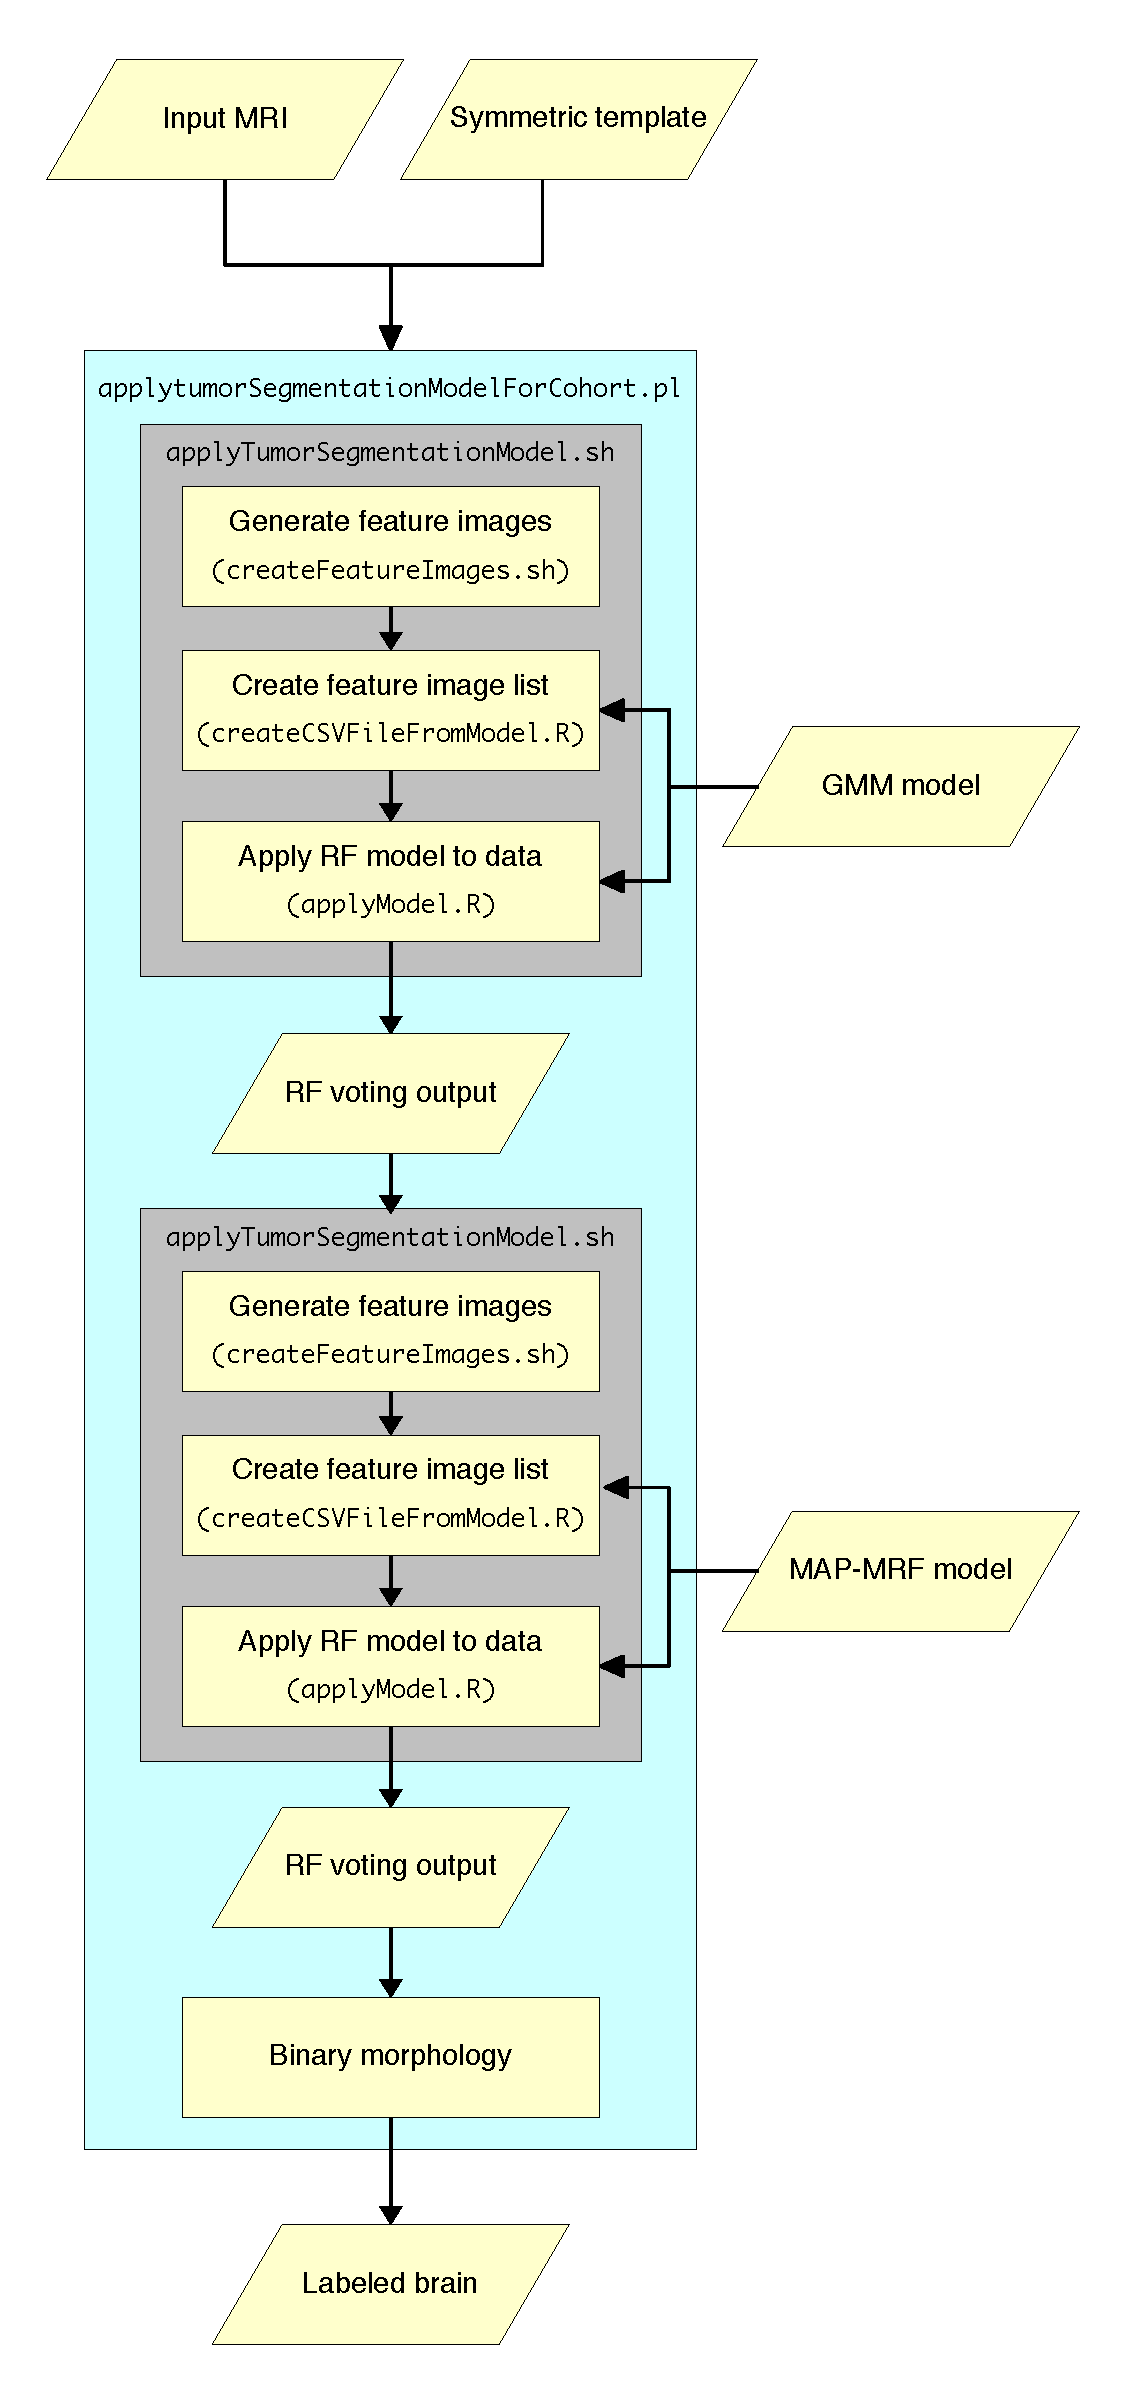
\includegraphics[width=85mm]{Figures/pipeline.pdf}
  \end{tabular}
  \caption{Diagrammatic workflow for the proposed RF model prediction.  The feature
  images are first generated from the input MRI and symmetric multivariate template. 
  After organization of the feature images in a csv file, the stage 1 RF model is 
  applied which results in a first stage classification voting output.  This output
  is used to generate an additional set of feature images for the second classification
  stage.  The final refinement process entails a series of binary morphological 
  operations which results in the final labeled brain.  In the diagram we also list
  the files used to perform each set of functions which are available as open source.
  }
  \label{fig:pipeline}
\end{figure}







\begin{figure*}
  \centering
  \begin{tabular}{cc}
  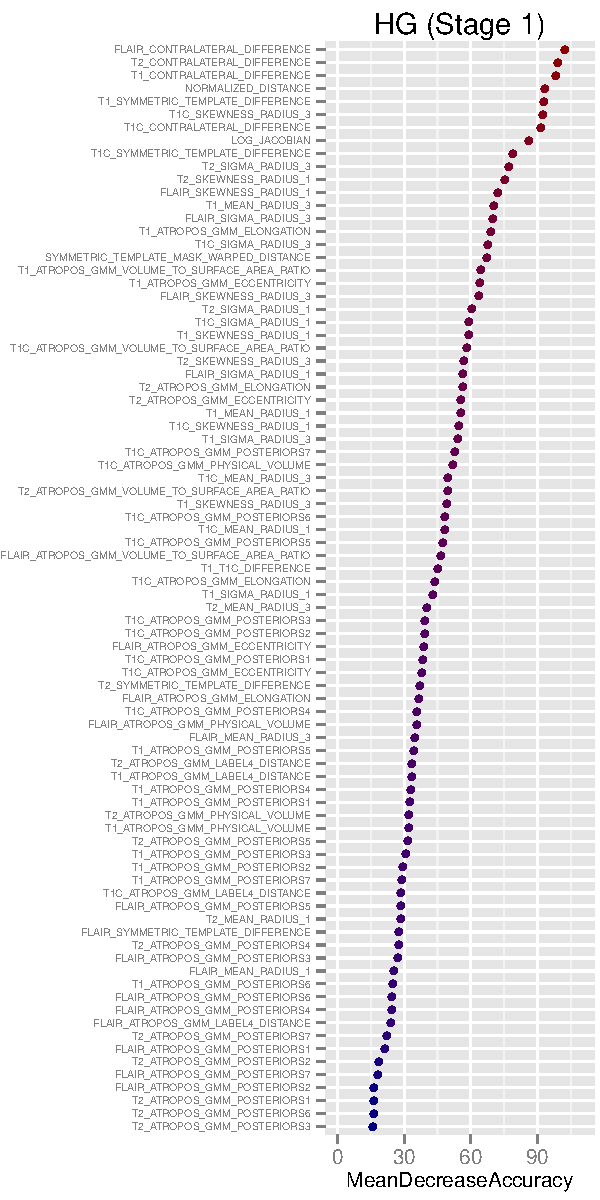
\includegraphics[width=80mm]{Figures/BRATS_HG_GMM.pdf} &
  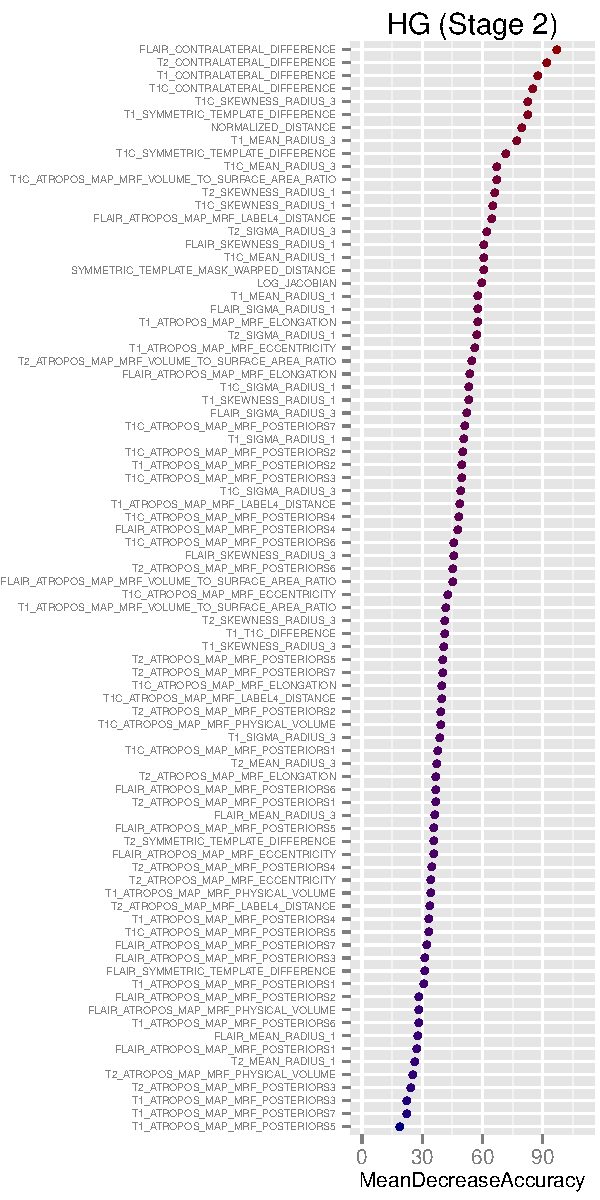
\includegraphics[width=80mm]{Figures/BRATS_HG_MAP_MRF.pdf} \\
  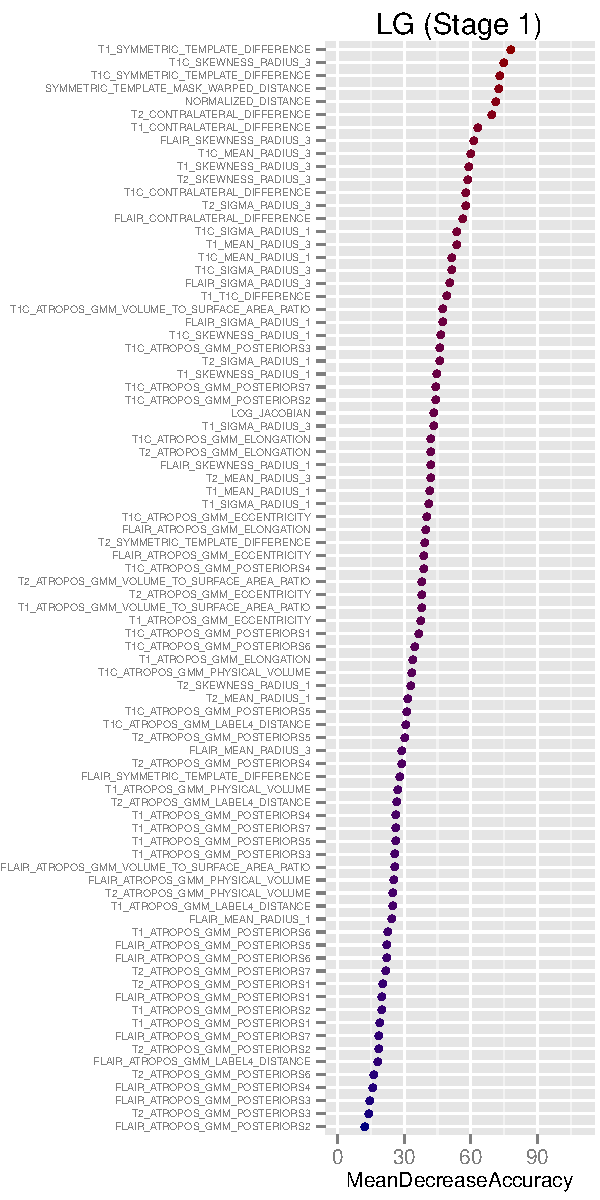
\includegraphics[width=80mm]{Figures/BRATS_LG_GMM.pdf} &
  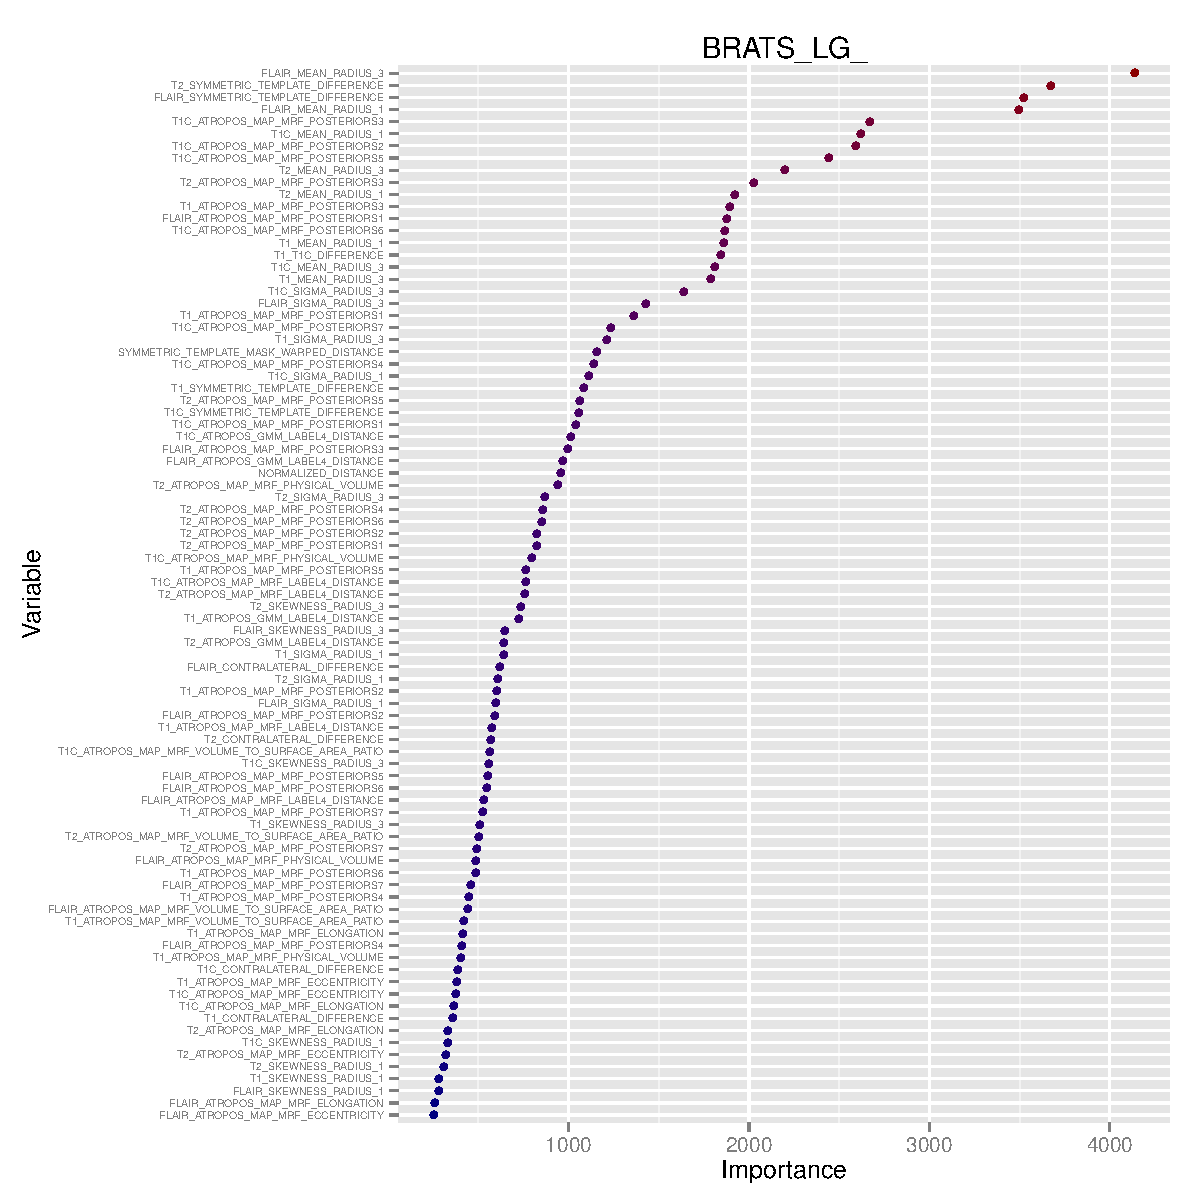
\includegraphics[width=80mm]{Figures/BRATS_LG_MAP_MRF.pdf}
  \end{tabular}
  \caption{Feature images from the BRATS\_HG0004 data set.}
\end{figure*}






\section{Results}

\begin{table*}
\caption{Dice scores from the MICCAI 2012 BRATs Study}
\begin{center}
\begin{tabular*}{0.975\textwidth}{@{\extracolsep{\fill} } c c c c c c c c c}
\toprule
{} & \multicolumn{2}{c}{High-grade (real)} & \multicolumn{2}{c}{Low-grade (real)} & \multicolumn{2}{c}{High-grade (simulated)} & \multicolumn{2}{c}{Low-grade (simulated)}\\
{\bf Method} & Edema & Tumor & Edema & Tumor & Edema & Tumor & Edema & Tumor\\
\midrule
\cite{zikic2012} & {$0.70 \pm 0.09$} & {$0.71 \pm 0.24$} & {$0.44 \pm 0.18$} & {$0.62 \pm 0.27$} & {$0.65 \pm 0.27$} & {$0.90 \pm 0.05$} & {$0.55 \pm 0.23$} & {$0.71 \pm 0.20$} \\
\cite{bauer2012} & {$0.61 \pm 0.15$} & {$0.62 \pm 0.27$} & {$0.35 \pm 0.18$} & {$0.49 \pm 0.26$} & {$0.68 \pm 0.26$} & {$0.90 \pm 0.06$} & {$0.57 \pm 0.24$} & {$0.74 \pm 0.10$} \\
ANTsR & {$0.65 \pm 0.15$} & {$0.66 \pm 0.28$} & {$0.49 \pm 0.16$} & {$0.65 \pm 0.21$} & {$0.68 \pm 0.25$} & {$0.91 \pm 0.08$} & {$0.61 \pm 0.25$} & {$0.84 \pm 0.09$} \\
w/ Atropos & {$0.68 \pm 0.15$} & {$0.67 \pm 0.30$} & {$0.50 \pm 0.15$} & {$0.67 \pm 0.23$} & {$0.74 \pm 0.26$} & {$0.92 \pm 0.09$} & {$0.65 \pm 0.26$} & {$0.84\pm 0.08$} \\
\bottomrule
\end{tabular*}
\end{center}
\end{table*}

\section{Discussion and Conclusions} 

%% References with bibTeX database:

%\section*{Acknowledgments}

\section*{References}

\bibliographystyle{elsarticle-harv}
\bibliography{references}


%% Authors are advised to submit their bibtex database files. They are
%% requested to list a bibtex style file in the manuscript if they do
%% not want to use model1-num-names.bst.

%% References without bibTeX database:

% \begin{thebibliography}{00}

%% \bibitem must have the following form:
%%   \bibitem{key}...
%%

% \bibitem{}

% \end{thebibliography}


\end{document}

%%
%% End of file `elsarticle-template-1-num.tex'.
